\section{Einleitung}

TODO

\section{Datenformat}

\noindent In der Datei {\tt bays29.tsp} sind 29 bayrische Städte aufgeführt.
Der Kern der Datei ist die 29x29 Matrix, welche die Reisekosten zwischen
den den einzelnen Städten beschreibt, dieser Städte-Graph ist zur Lösung
des Travelling-Salesman-Problems (TSP) gedacht.
Details des Aufbaus der Datei:

\begin{itemize}
  \item Header.\\
  Name, Problemtyp, Kommentar, Dimension des Problems bzw. der Matrix, Typ und Format der Kantengewichte
  \item Kantengewichte.\\
  29 x 29 Matrix mit den Reisekosten zwischen den einzelnen Städten als symmetrische Matrix, d.h. es handelt sich um einen ungerichteten Graphen.
  \item Positionen der Städte.\\
  Liste mit Stadtnummer und X-, Y-Koordinaten, welche die Städtepositionen beschreiben.
  Diese Informationen sind lediglich zur Visualisierung (Matlab Plot) nötig.
\end{itemize}


\section{Testläufe mit tspVorlage.m}

Das {\tt tspVorlage.m} Skript wurde 15 mal ausgeführt und die Ergebnisse in
Tabelle \ref{testlaeufe} festgehalten und auf Abbildung \ref{fig.testlaeufe}
visualisiert.
Eine kleine Auswertung ergibt einen Mittelwert von 3077.93 km mit
einer Standardabweichung von 177.05 km.
Das Minimum beträgt 2764 km und das Maximum 3490 km.

Laut \cite{aufg} liegt die beste
Lösung\footnote{In der Software \emph{best objective value} genannt.},
also der kürzeste Weg für eine Rundreise, bei 2020 km.
Das bedeutet, hier gibt es noch Optimierungsbedarf.
In den Kapiteln \ref{populations} bis \ref{mutation} werden systematisch bessere Einstellungsparameter
gesucht, um einen möglichst kurzen Weg mit möglichst geringer Laufzeit zu finden.

\begin{table}[h]
\begin{tabular}{ | r | c | c | }
  \hline
  \# Iteration & kürzester Weg & in Generation \\
  \hline
  1  & 3324 & 288 \\
  2  & 3041 & 345 \\
  3  & 3180 & 388 \\
  4  & 3148 & 244 \\
  5  & 3102 & 372 \\
  6  & 2898 & 243 \\
  7  & 2980 & 287 \\
  8  & 2764 & 139 \\
  9  & 2982 & 307 \\
  10 & 3490 & 319 \\
  11 & 2974 & 293 \\
  12 & 3281 & 364 \\
  13 & 2991 & 313 \\
  14 & 2967 & 261 \\
  15 & 3047 & 353 \\
  \hline
\end{tabular}
\caption{Testläufe mit {\tt tspVorlage.m}}\label{testlaeufe}
\end{table}

\begin{figure}[h!]
  \centering
  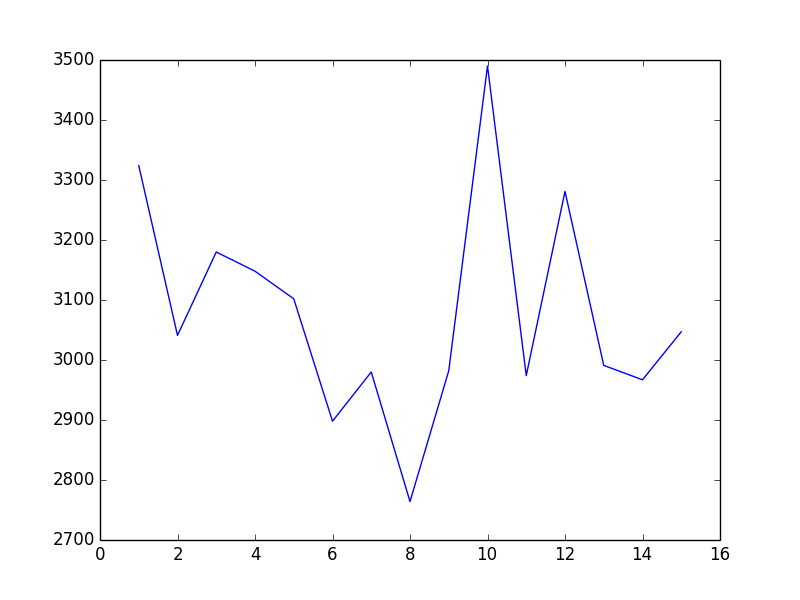
\includegraphics[width=1.0\textwidth]{Figures/gen/tspVorlage.png}
  \caption{Testläufe mit {\tt tspVorlage.m}}\label{fig.testlaeufe}
\end{figure}


\section{Parameter und Optionen}

Mit der Methode {\tt geaoptset( Key, Value )} können beliebig viele
Parameter an den evolutionären Algorithmus übergeben\footnote{Natürlich
muss der Algorithmus diese Parameter auch verarbeiten können.} werden.
Eine nochmalige Zuweisung des {\tt Key} überschreibt den {\tt Value}.
Im Folgenden sollen die ausschlaggebenden Parameter und
ihre Auswirkungen griffig beschrieben werden.

% TODO: Intervalle der Voreinstellungen aufschreiben.
% TODO: ggf. genauere Beschreibungen von der Doku übernehmen

\paragraph{{\tt VariableFormat}} Die Option definiert das Format der Variablen
und die Konvertierung zwischen der internen Repräsentation (Genotyp) und dem
Phänotyp.
Voreinstellung: 5 (Ordnungs- \& Permutationsprobleme).

\paragraph{{\tt NumberSubpopulation}} Gibt die Anzahl der Unterpopulationen an.
Bildlich gesprochen: die Anzahl der Indianerstämme.
Voreinstellung: 1.

\paragraph{{\tt NumberIndividuals}} Regelt die Anzahl
der Individuen, welche pro Unterpopulation existieren.
Voreinstellung: 50.

\paragraph{{\tt Selection.Name}} Legt fest mit welcher Funktion Individuen
aussortiert werden, welche also nicht mehr in die nächste Generation
übernommen werden.
Voreinstellung: selrws (Roulette Wheel Selection).

\paragraph{{\tt Selection.GenerationGap}} Anteil der Population, welcher pro
Generation reproduziert wird.
Voreinstellung: 1 (=100 Prozent).

\paragraph{{\tt Recombination.Name}} Regelt mit welcher Fortpflanzungsmethode
sich Individuen kreuzen.
Voreinstellung: recpm (Partially matched Crossover).

\paragraph{{\tt Mutation.Name}} Legt fest mit welcher Funktion eine Mutation
an einem Individuum durchgeführt wird.
Voreinstellung: mutswap (mutation by swapping variables).

\paragraph{{\tt Mutation.Rate}} Gibt die Anzahl der Mutationen
pro Individuum an.
Voreinstellung: 10.

\paragraph{{\tt Termination.MaxGen}} Gibt an, wie viele Generationen der
Algorithmus berechnen soll.
Voreinstellung: 400.

\paragraph{{\tt Termination.Method}} Legt fest mit welcher Methode der
Optimierungsalgorithmus beendet werden soll.
Voreinstellung: 1 (Beenden nach der maximalen Anzahl der Generationen).

\paragraph{{\tt Output.*}} Diese Parameter sorgen für die
Ausgabe\footnote{In Form vom Plots, Standard-Out und Dateien.} der Resultate,
jedoch sind diese nicht relevant, da das in Kapitel \ref{testsystem} beschriebene
automatisierte Testsystem all diese Aufgaben übernimmt.

\paragraph{{\tt [xnew, GeaOpt] = geamain2(objfun, GeaOpt, VLUB, []);}}
Hauptfunktion die zwei Datenstrukturen zurückgibt, wobei folgende
Informationen von besonderem Interesse sind:

\begin{itemize}
  \item Der beste Weg: {\tt xnew(1,:)}
  \item Länge des kürzesten Weges: {\tt GeaOpt.Run.BestObjectiveValue}
\end{itemize}

